\section{Winding Numbers and Cauchy's Integral Formula}

\begin{lemma}\label{4.5.1}
    Let $\y:[0,1] \xrightarrow{} \C$ be a closed rectifiable path. Define, for
    $z_0 \notin \{\y\}$ the path integral
    \begin{equation*}
        W=\frac{1}{2i\pi}\int_\y{\frac{dz}{z-z_0}}
    \end{equation*}
    Then $W \in \Z$.
\end{lemma}
\begin{proof}
    Suppose, without loss of generality, that $\y$ is of class  $C^1$. Define
    $g:[0,1] \xrightarrow{} \C$ by
    \begin{equation*}
        g(t)=\int_0^t{\frac{\y'(s)}{\y(s)-z_0} \ ds}
    \end{equation*}
    hence $g(0)=0$ and $g(1)=\int_\y{\frac{dz}{z-z_0}}$. Moreover, notice that
    \begin{equation*}
        g'(t)=\frac{\y'(s)}{\y(s)-z_0} \text{ on } 0 \leq t \leq 2\pi
    \end{equation*}
    Then we get $D{(\exp{(-g)(\y-z_0)})}=0$ so that $\exp{(-g)(\y-z_0)}$ is the
    constant function, and
    $\exp{(-g)(\y(0)-z_0)}=\exp{(-g)(\y(1)-z_0)}=2i\pi{k}$, and $k \in \Z$.
    Notice that $k$ is precisely $W$.
\end{proof}

\begin{definition}
    Let $\y$ be a rectifiable closed path in  $\C$. We define the
    \textbf{winding number} of $\y$  \textbf{around} some point $z_0 \notin
    \{\y\}$ to be the path integral given by
    \begin{equation*}
        W(\y,z_0)=\frac{1}{2i\pi}\int_\y{\frac{dz}{z-z_0}}
    \end{equation*}
\end{definition}

\begin{lemma}\label{4.5.2}
    If $\y$ and $\s$ be closed rectifiable paths having the same initial points.
    Then the following are true
    \begin{enumerate}
        \item[(1)] $W(\y,z_0)=-W(\y^-,z_0)$ for all $z_0 \notin \{\y\}$.

        \item[(2)] $W(\y+\s,z_0)=W(\y,z_0)+W(\s,z_0)$ for all $z_0 \notin \{y\}
            \cup \{\s\}$.
    \end{enumerate}
\end{lemma}

\begin{definition}
    Let $\y$ be a closed path. We define the \textbf{interior} of $\y$ to be the
    open set  $U$ of $\C$ having as boundry the trace  of $\y$, i.e.
    $\partial{U}=\{\y\}$. We denote the interior of $\y$ by $\Int{\y}$. We call
    an open set $U$ of the set $\com{\C}{\{\y\}}$ a component \textbf{bounded}
    by $\y$ if $U \subseteq \Int{\y}$, and \textbf{unbounded} otherwise.
\end{definition}

\begin{figure}[h]
    \centering
    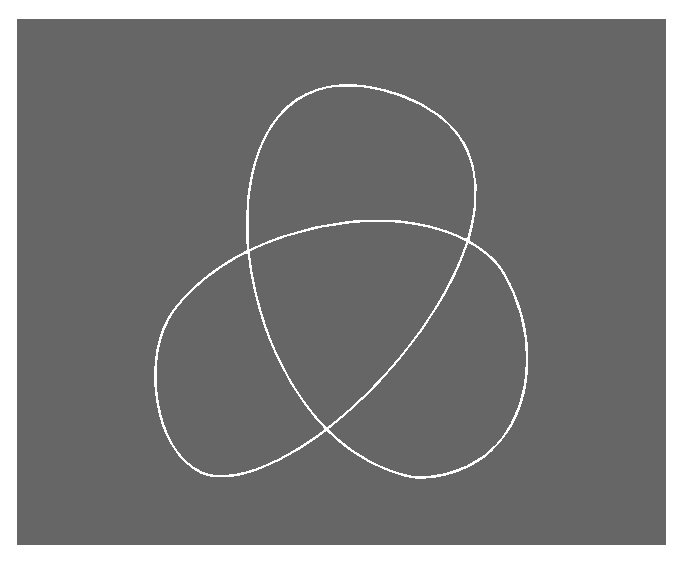
\includegraphics[scale=0.5]{Figures/Chapter4/bounded_components.eps}
    \caption{A closed rectifiable path $\y$ with its bounded components. Notice
    that the component lying outside of $\{\y\}$ is an unbounded component.}
    \label{fugure_4.2}
\end{figure}

\begin{theorem}\label{4.5.3}
    Let $\y$ be a closed rectifiable path in  $\C$. Then  $W(\y,z_0)$ is
    constant for any $z_0$ in a component $U$ of  $\com{\C}{\{\y\}}$. Moreover,
    if $z_0$ is in an unbounded component, then  $W(\y,z_0)=0$.
\end{theorem}
\begin{proof}
    Let $f:U \xrightarrow{} \C$ be defined by $f(z)=W(\y,z)$. Now, fix a $z_0
    \in U$, and let $r$ be the distance between  $z_0$ and $\{\y\}$. If
    $|a-b|<\d<\frac{r}{2}$, then we  get
    \begin{equation*}
        |f(a)-f(b)|=
        \frac{1}{2i\pi}\Big{|} \int_\y{\frac{a-b}{(z-a)(z-b)} \ dz} \Big{|} \leq
        \frac{|a-b|}{2i\pi}\int_\y{\frac{|dz|}{|z-a||z-b|}}
    \end{equation*}
    now, for $|a-b|<\frac{r}{2}$, and $z \in \{\y\}$, we get $|z-a| \leq
    r>\frac{r}{2}$, thus $|f(a)-f(b)|<\frac{2\d}{\pi{r^2}}V(\y)$ so if $\e>0$,
    choosing  $\d<\min{\{\frac{r}{2}, \frac{\pi{r^2}}{2V(\y)}\}}$, and we get
    that $f$ is continuous.

    Now, if $U$ is a component of $\com{\C}{\{\y\}}$, then $f(U)$ is connected.
    However, notice that $f(U) \subseteq \Z$, so that $f(U)$ must be pointset.
    Therefore $f$ is constant on $U$.

    Now, let $V$ be an unbounded component of $\com{\C}{\{\y\}}$; i.e. $V
    \notsubseteq \int{\y}$; then there exists an $R>0$ such that the set  $\{z
    \in V : |z|>R\} \subseteq V$. If $\e>0$, choose a point  $z_0$ with
    $|z_0|>R$, and $|z-z_0|>\frac{V(\y)}{2\pi\e}$ uniformly for $z \in
    \{\y\}$. Then $|W(\y,z_0)|<\e$ so that $W(\y,z_0) \xrightarrow{} 0$. Since
    $W(\y,z_0)$ is constant, this makes $W(\y,z_0)=0$ on $V$.
\end{proof}
